\chapter{Datenbeschaffung und Speicherung}\label{ch:data}

\section{Ausgangslage}

Um eine Zusammenstellung verschiedener Audiosegmente möglichst genau und inhaltlich abgestimmt auf ein bestimmtes Thema zu fokussieren, müssen auch zu diesem Thema passende Audioabschnitte in den Daten verfügbar sein.
Als Audiodaten könnten fast alle Audioressourcen genutzt werden, wie zum Beispiel Beiträge aus Radioprogrammen, die Audiospuren von Videos oder ganze Podcasts Episoden.

Die Qualität dieses Systems würde mit steigender Anzahl an Audiomaterial auch bessere Ergebnisse erzielen, allerdings ist es im Umfang dieser Arbeit nicht möglich alle Daten als Audiomaterial zu verwenden.
Die Audiodaten müssten dazu erst transkribiert werden und anschließend mit diesen Transkripten Embeddings generiert werden, was Zeit- und Ressourcenintensiv ist.
Für diese Arbeit wurde versucht möglichst qualitativ hochwertige Daten zu benutzen, um mit den möglichen Ressourcen und in gegebener Zeit einen qualitativ hochwertigen Prototypen zu erstellen. 

Als Audiomaterial würde sich am besten Podcasts eignen, 
Die beste Audioquelle wäre Audiomaterial, in dem über verschiedene Themen sachlich gesprochen wird, die Informationen aber gleichzeitig faktisch korrekt wären.
Außerdem sollten die Audioquellen frei verfügbar sein, damit keine Urheberrechtsverletzung stattfindet.

% Eine Garantie für Sachlichkeit und 

% Es sollten nicht die Vortragenden Personen wichtig sein  und sie nicht emotional oder persönlich 
% Als Audioquelle kommen vor allem wissensbasierte Podcasts in Frage, 
% Wissensbasierte Podcasts bieten als Audioform die besten qualitativen Inhalt für die Audiosegmente, wenn sie 
% Die Audioform mit dem meisten 

% Als Anbieter von Audiomaterial bieten sich zum Beispiel YouTube oder Spotify an, die sehr viele 


% Am besten 

% Für die Grundlage der Audiosegmente bieten sich insbesondere wissensbasierte Podcasts an, die den Zuhörenden Informationen vermitteln wollen, wenn sie 


% Videos wie zum Beispiel von Youtube, setzen oft vorraus, dass der Zuschauer auch das Videomaterial sehen kann und somit würde nur das Hören der Audiospur zu verwirrung führen.

%  im gegensatz zu Radioprogrammen keine Musik
% Die Podcastbranche wächst seit vielen Jahren stetig und immer mehr Menschen hören regelmäßig Podcasts.
% In Deutschland schon über 29\%.
% Genauso wächst auch die Anzahl an verschiedenen Podcasts.

% Daraus kann man ableiten, dass  

\section{Die ARD-Audiothek}

Die ARD-Audiothek ist in Deutschland eine der gößten Audio- und Podcastanbieter mit mitlerweile über 41 Millionen Audioabrufen und über 100.000 verschiedenen verfügbaren Audioinhalten. 
Die Inhalte unterliegen alle den journalistischen Grundsätzen der ARD und bieten somit einen sorgfältigen Qualitätsstandard. 
Die verschiedenen Audioinhalte stammen von den einzelnen Landesrundfunkanstalten, der ARD und dem Deutschlandradio und liefern eine Vielzahl verschiedener Inhalte.
Sie enthält über 2000 verschiedene Podcasts, in vielen unterschiedlichen Kategorien, wie Comedy, Sport, Wissenschaft, Wirtschaft, Gesellschaft, Kunst, Musik oder Philosophie. 
In dieser Audiothek gibt es zudem Hörbücher, Hörspiele, oder Podcasts nur für Kinder.
Die einzelnen Rundfunkanstalten tragen außerdem eigene Podcasts bei, die meist einen regionalen Kontext haben, wie zum Beispiel der Podcast "Giga Grünheide" über das Teslawerk in Brandenburg vom rbb
Alle diese Inhalte sind kostenlos und frei verfügbar und stellen eine gute Quelle für das Audiomaterial dar, das in dieser Arbeit verwendet wird.




% Im Appstore und im Google Playstore hat die App der ARD-Audiothek jeweils über eine Million Downloads.
% \cite{gotting2023}




\section{Podcastreihe Radiowissen}

Zur automatischen Generierung von Podcast Episoden bietet es sich an, dass in den Ausgangsaudios die Sprache klar und verständlich ist und verschiedene Sprecher sich nicht ins Wort fallen bzw. gleichzeitig reden.
Außerdem ist es wünschenswert, die ausgeschnittenen Audiosegmente an klaren Satzgrenzen zu teilen, sodass der Ausschnitt nicht mitten im Satz beginnt und dem Zuhörenden der Kontext vorenthalten wird. 

Als Datengrundlage wird die Podcastreihe Radiowissen von bayern2 benutzt. 
Diese ist nicht wie ein klassischer Podcast im Dialogstil aufgebaut, sondern ähnlich wie bei einem Hörspiel wird der Text von einem Manuskript abgelesen. 
Dazu kommen verschiedene Geräusche und verschiedene Stimmen, um dem Hörenden mehr Abwechselung zu bieten.

Der Fokus der einzelnen Episoden liegt auf interessanten Beiträgen zu verschiedenen Themen, die häufig Gebiete der Geschichte, Naturwissenschaft, Gesellschaft oder Philosophie umfasst.
Beispielepisoden sind: "Fasten - Verzicht und innerer Gewinn?", "Die Maus - Anpassungskünstler und gefürchteter Schädling", oder "Maria Sibylla Merian - Naturforscherin und Künstlerin".

Die mehr als 2000 Episoden wurden von mehr als 150 verschiedenen Autoren geskriptet.
Dadurch sind die einzelnen Episoden unterschiedlich in der Erzählweise.
In einigen Episoden kommen originale Audiospuren von historischen Aufnahmen vor oder auch  Gastbeiträge von Experten. Zudem wird beinahe jeder Podcast abwechselnd von mehreren Stimmen vorgetragen, was nachweislich die Aufmerksamkeit von Zuhörenden verbessert \cite{kang2012}.

\section{Datenbeschaffung über die ARD-Audiotheks API}

Die Inhalte der ARD-Audiothek kann man entweder direkt über die Webseite erreichen oder mithilfe einer frei benutzbare Web-GraphQL API abfragen.
(https://api.ardaudiothek.de/graphql) 
Über diese Schnittstelle sind alle Informationen, wie Titel, Beschreibungen, Autoren oder auch der Link zu dem MP3-File jeder Episode abrufbar.

Über die GraphQL-Abfrage \autoref{ch:graphql-1} erhält man alle Download-Links zu den Podcast-Episoden des Podcasts "Radio Wissen" von bayern2.
Das sind (Stand 3. Januar 24) 2257 Podcast Episoden.

Alle diese Audiodatein wurden anschließend heruntergeladen und auf einer lokalen Festplatte gespiechert.
Dabei kam es insgesamt 15 mal vor, dass zwei Episoden den selben Titel tragen, aber eine unterschiedliche Download-URL aufwiesen.
Die URL unterschieden sich nur, indem hinten die Zeichen "-1" oder "-2" angefügt wurden.
Zum Beispiel hat die Episode "Quantenphysik - Wahr, aber verrückt" den Downloadlink https://media.neuland.br.de/file/1804047/c/feed/quantenphysik-wahr-aber-verrueckt.mp3 aber auch https://media.neuland.br.de/file/2069613/c/feed/quantenphysik-wahr-aber-verrueckt-1.mp3.
In diesem Fall liefert nur die zweite URL einen Download, die erste zeigt eine Fehlermeldung an.
Es gibt auch Fälle in denen beide Links funktionieren, wie zum Beispiel 
https://media.neuland.br.de/file/32891/c/feed/die-bamberger-hexenprozesse-unschuldig-muss-ich-sterben.mp3 und
https://media.neuland.br.de/file/1858845/c/feed/die-bamberger-hexenprozesse-unschuldig-muss-ich-sterben-1.mp3   
Die Daten wurden dementsprechend bereinigt und doppelte Audioinhalte nur einmal abgespeichert.

Für weitere Analysen und die Kategorisierung der Audiodatein ist es außerdem Sinnvoll, die Beschreibungen der einzelnen Episoden und die dazugehörenden Schlagwörter abzufragen, da diese eine Kurze Zusammenfassung oder Einordnung der Episoden enthalten.
Über das Entstehungsdatum können des witeren Informationen später nach Aktualität gefiltert werden 
Über die Anfrage \autoref{ch:graphql-2} können all diese Informationen abgefragt werden.

Über die API kann auch in einigen Fällen direkt ein Transkript des Audiofiles angefordert werden. 
Allerdings ist die Transkription meist nicht sehr akkurat.
Nähreres dazu in Kapitel \autoref{ch:method}


\section{Datenanalyse}

Die 2232 einzigartigen Episoden haben eine durchschnittliche Länge von 22 Minuten und einen durchschnittlichen Größe von 21 MB.
Insgesamt weisen diese Audiodaten eine Größe von ungefähr 47 GB auf. 

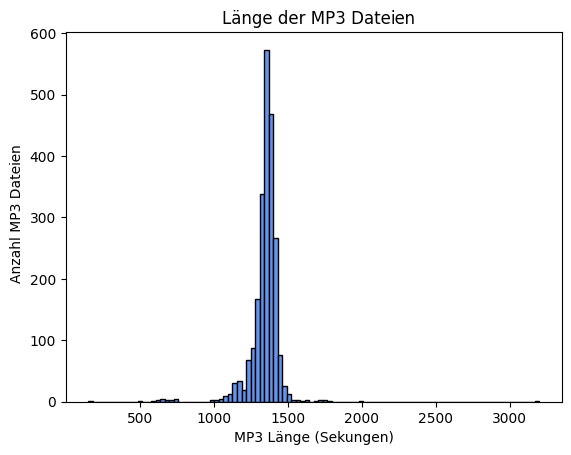
\includegraphics[width=\linewidth]{figures/mp3_length.png}

Der kürzeste Podcast ist "ab-jetzt-in-der-ard-audiothek-kinder-der-flucht-frauen-erzaehlen.mp3", der nur 2 Minuten 30 Sekunden lang ist und ein Teaser für einen anderen Podcast darstellt.
Die längste MP3 Datei ist mit Abstand "deportation-und-exil-eine-polnische-odyssee-im-zweiten-weltkrieg.mp3" mit einer Länge von mehr als 53 Minuten.
Diese Episode ist mehr als doppelt so lang wie eine durchschnittliche Episode und bildet einen Ausnahmefall.

Die 




\section{Datenspeicherung}

\subsection{Datenspeicherung SQLite}

Für die Analyse werden die MP3-Dateien der einzelnen Podcast-Episoden in einem seperaten Ordner gespeichert und die Benennung der originalen Dateien stammt aus der URL.
Zur Speicherung der Transkripte wird das relationale Datenbank Managment System (RDBMS) SQLite  eingesetzt. SQLite ist für Datenanalysezwecke sehr gut geeignet, weil es simpel und performant ist und als opensource-Projekt kostenlos verwendet werden kann.
Im Gegensatz zu anderen RDBMS, wie mySQL oder PostgreSQL arbeitet SQLite serverunabhängig und speichert alle Tabellen in einer einzigen Datei, was sehr nützlich für den Datenaustausch zwischen verschiedenen Geräten ist.
Für einige Operationen, wie die Transkription der Audiodateien oder die Generierung von Embeddings wird die Hardware eines High-Performance Clusters der Technischen Hochschule Nürnberg genutzt. 
Um die Daten zu analysieren und zu nutzen bietet es sich an, auf Consumer-Hardware zu wechseln und dafür ist eine gute Portabilität der Datenbank von Vorteil.

SQLite unterstützt Datenmengen bis zu 140 TB. 
Allerdings wird auf der offiziellen Webseite angegeben, dass ab einer Größe von 1 TB auf serverbasierte RDBMS umgestiegen werden sollte, da die gesamte Datenbank in einem File gespeichert wird und viele Client-Betriebssysteme eine maximale Größe der Dateien vorgeben. 
Falls das Projekt in der Zukunft auf mehrere Podcast-Reihen ausgeweitet wird, sollte vor diesem Hintergrund ein Wechsel des DBMS in Betracht gezogen werden.

\subsection{Datenspeicherung Vektoren SQLite}

Da SQlite nativ keine Listen oder Tabellen als Einträge in einer Datenbank speichern kann, ist es nicht trivial, die Embeddings abzuspeichern.
Zunächst wurde die Möglichkeit in Betracht gezogen, jeden einzelnen Eintrag aus einem Embedding-Vektor als seperaten Eintrag in einer Tabelle zu speichern. 

Das führt allerdings zu sehr ineffizienten Abfragen der Daten und beim Einfügen von Daten limitiert SQLite die Anzahl der Parameter, sodass längere Embeddings umständlich gestückelt abgespeichert werden müssten.

Als Nächstes wurde überprüft, ob man die Embeddings als serialisiertes Array abspeichern kann.
Dafür wurde jedes Embedding in einen JSON-String umgewandelt, der dann gespeichert werden soll. 
Dabei tritt leider das Problem auf, dass die Daten bei der Verwendung wieder deserialisiert werden müssen.
Dieser Schritt müsste jedes Mal wiederholt werden, wenn eine Suche stattfindet. 
Dies dauert sehr lange und ist sehr ineffizient. 
Für die deserialisierung von 400.000 Sätzen mit einem 384 dimensionalen Embedding eines Sentence Transformer Modells auf einem Intel i7 Quad-Core beträgt die Rechenzeit ca. 45 Min.

Zur Datenspeicherung der Embedding-Vektoren muss zwischen Dense- und Sparce-Vektoren unterschieden werden, da für beide Embedding-Methoden unterschiedliche Optimierungen in der Speicher und Retrival Funktionalität vorliegen. 

\subsection{Datenspeicherung Dense Vektoren}

Um Dichte-Vektoren abzuspeichern, bietet es sich an, eine seperate Vektordatenbank zu nutzen.
Eine Vektordatenbank ist eine nichtrelationale Datenbank, die darauf spezialisiert ist, eine effiziente Suche in ungeordneten Informationen zu ermöglichen.
Dazu speichert sie die Embedding-Vektoren verschiedener Datenquellen effizient ab und erlaubt Zugriff auf schnelle Suchalgorithmen, wie Approximate Nearest Neighbour Algorithmen.

Es gibt verschiedene Approximate Nearest Neighbour Algorithmen, die alle darauf abzielen, den gesamten Suchraum für eine Ähnlichkeitssuche in kleinere Unterräume aufzuteilen.
Dabei werden oft Baum-Strukturen verwendet, um die Suche effizienter zu gestalten.
Speziell Algorithmen wie Hierarchical Navigable Small Worlds werden von vielen Vektordatenbanken benutzt.

% Vektordatenbanken entwickeln sich in den letzten Jahren stark weiter.
% In diesem Projekt wurde zunächst die Vektordatenbank Milvus betrachtet.
% Milvus kann sehr gut auf große Datenmengen skalieren und wird deshalb in vielen großen Unternehmen, wie Nvidia, Paypal oder ebay eingesetzt. 
% Außerdem bietet Milvus Unterstützung für eine clusterbasierte Struktur, in der einzelne Container dynamisch zusammenarbeiten können. 
% Dadurch wird eine gute Skalierbarkeit für große Datenmengen erreicht. 
% Für kleinere Projekte ist der Setup-Aufwand sehr groß und die Lernkurve sehr steil.

% Pinecone, Zilliz, Qdrant

% Außerdem gibt es eine Erweiterung für die PostgreSQL Datenbank namens pg-Vector

% Die Vektordatenbank Redis

% Durch die Neuheit der Vektordatenbanken bedingt, gibt es kaum Vergleiche zwischen diesen.
% \cite{blueteamai}


% In dieser Arbeit wird die Vektordatenbank Milvus verwendet.
% Milvus ist eine Open-Source Vektordatenbank die von dem Unternehmen Zilliz entwickelt wird.
% Laut eigenen Angaben ist sie die am weitseten fortgeschrittene Vektordatenbank und wird von vielen Unternehmen, wie Nvidia, Paypal oder ebay benutzt.

In dieser Arbeit wird die Vektordatenbank Chroma verwendet. 
Chroma ist eine einfache Vektordatenbank, die die Daten sowohl lokal als auch über eine Client-Server-Schnittstelle speichern kann.
Das Projekt ist erst im Mai 2022 als Startup entstanden, verfügt aber mittlerweile über viele Features, die die Datenverwaltung erheblich vereinfachen.
Die Datenbank ist dabei mit einer NoSQL-Datenbank zu vergleichen, indem die Daten nicht relational in Tabellen gespeichert werden, sondern in einer Collection als Objekte mit verschiedenen Metadaten.
Jedes dieser Objekte hat eine Document-Eigenschaft, welche den Inhalt des Dokuments repräsentiert.
Dieser Inhalt ist in diesem Fall ein Ausschnitt aus einem Transkript, könnte aber auch ein Bild oder eine Audiodatei darstellen.

Außerdem besitzt jedes Objekt einen Embedding-Vektor, der mit dem Dokument assoziiert wird. 
Innerhalb einer Collection müssen alle Objekte mit der selben Embeddingmethode encodiert werden.
Das sichert die Vergleichbarkeit der verschiedenen Vektoren untereinander.

ChromaDB bietet nativen Support für verschiedene Embedding Modelle von OpenAI, Huggingface, Cohere, instructorembedding und JinaAI.
Dafür müssen nur das Model und der plattformspezifische API-KEY angegeben werden und Chroma erstellt automatisch für jedes Dokument das Embedding.
Standardmäßig ist das Embedding des Sentence Transformer Modells all-MiniLM-L6-v2 eingestellt.
Alternativ können auch schon vorgefertigte Embeddings eingefügt und die dazugehörige Embedding Funktion eingetragen werden.
In dieser Arbeit wurden die Embeddings von OpenAI und all-MiniLM-L6-v2 schon vorher erstellt und dort eingetragen.

Chroma bietet außerdem sehr guten Support für effizientes Retrieval von Dokumenten.
Dazu sind schon verschiedene verfahren der Nearest Neighbour Suche implementiert.
 

In diessem Projekt wurde erst in einer späten Phase der Umstieg auf die Vektor-Datenbank vollzogen, weshalb einige Funktionen, die in dieser Datenbank automatisch integriert sind, noch einmal sehr ausführlich beschrieben werden.


\subsection{Datenspeicherung Sparce Vektoren}

Chroma bietet leider noch keine Unterstützung zur Speicherung von Sparce Vektoren.
Stattdessen wurde das Python-Modul pickle verwendet, welches darauf spezialisiert ist, Python Objekte effizient als Bytecode zu serialisieren. 
Es bietet auch die Möglichkeit, Datenstrukturen effizient zu speichern bzw. zu laden und hat seit Python 3.8 auch guten Support, um große NumPy Arrays effizient zu speichern, was zuvor nur mit der joblib Bibliothek möglich war.
Pickle speichert die Daten in einem Python spezifischen Format ab, was die Portierbarkeit auf andere Systeme stark einschränkt. Dieses Format erlaubt es aber verschiedene Eigenschaften besser zu speichern als JSON (z.B. Pointer sharing).

Für den TF-IDF Algorithmus, bei dem ein Vokabular von mehr als 200.000 Wörtern eine ebensogroße Dimensionalität der Embeddingvektoren benötigt, würde ein normaler Serialisierungsalgorithmus für die 300.000 Sätze ca 60 Milliarden Werte abspeichern.
Wenn man für jeden dieser Werte eine 32 Bit Gleitkommazahl als Datentyp abspeichern würde, käme man auf ca. 240 GB Daten. 
Ein Großteil dieser Werte (~99,9\%) sind dabei 0.
Ein Numpy Array kann diese Werte sehr effizient zusammenfassen und mithilfe von pickle kann dieses kompakte Array effizient abgespeichert werden, wodurch eine tatsächliche Speichergröße von ca. 50 MB entsteht.
Dies ermöglicht auch ein effizientes laden und vergleichen der Embeddings, was für 400.000 Sätze auf einem Intel Quad-Core i7 ca. 1 Sekunde benötigt.

In der Zukunft könnte dieser Schritt durch einen Umstieg auf eine Plattform wie Elasticsearch vereinfacht werden.



% \subsection{weitere Schritte}


% Eine bekannte Bibliothek für Nearest Neighbour Searches ist Annoy, die unter anderem bei Spotify für die Recommendations von Songs verwendet wird. [Quelle]
% Eine weitere bekannte bekannte Bibliothek für Nearest Neighbour Searches ist FAISS (Facebook AI Similarity Search)

